\section{Przetwarzanie danych}
\subsection{Big Data}
Lawinowo rosnąca liczba nowych urządzeń podłączanych do sieci
oraz wzrost tempa generowania danych przez nie spowodowało,
że konieczne się stało stworzenie nowych metod ich analizy.
Klasyczne metody polegające na tworzeniu coraz większych,
mocniejszych komputerów (\textit{vertical scaling})
mierzących się z problemami analizy danych stawały się nie wystarczające.
Głównie ze względów ekonomicznych.
Takie rozwiązania były bardzo kosztowne w utrzymaniu i szybko stawały się przestarzałe.
Trzeba było szukać pomysłów w innym miejscu.
Zaczęto łączyć mniejsze komputery razem (\textit{horizonal scaling}),
by mogły rozwiązywać większe problemy.
Pojawiły się pierwsze rozwiązania gridowe,
obliczenia chmurowe (\textit{cloud computing})
czy mechanizmy typu \textit{MapReduce}.
Tematykę oraz wszystko co było w okół niej,
związana z masową analizą danych nazwano \textit{Big Data}.

Dane \textit{Big Data} można w skrócie opisać modelem \textit{3V} (Gartner Inc., 2012):
\begin{itemize}
		\item \textbf{Volume} - ilość,
		której nie można przetworzyć z wykorzystaniem standardowych metod i narzędzi.
		\item \textbf{Velocity} - zmienność.
		Dane napływają z różną częstotliwością (natężeniem),
		często w tym samym momencie.
		\item \textbf{Variety} - różnorodność.
		Dane pochodzą pochodzą z wielu źródeł.
		Mogą być lub nie ustrukturyzowane,
		w różnych formatach,
		wymagać wcześniejszego przeprocesowania,
		etc..
\end{itemize}

Obecnie rozwiązania \textit{Big Data} są coraz chętniej wykorzystywane przez firmy.
Począwszy od branży e-commerce,
gdzie są wykorzystywane między innymi do analizy behawioralnej klienta czy prognozowania zachowań,
do nawet bezpieczeństwa narodowego
na przykład NSA i program typowania terrorystów.

Główną cechą mechanizmów analizy \textit{Big Data} jest podział zadania
na wiele mniejszych,
niezależnych od siebie pod-zadań,
które mogą wykonywać się równolegle.
Dzięki dekompozycji zadania na niezależne pod-zadania,
można niskim kosztem zwiększać wydajność (\textit{throughput})
czy odporność na awarie (\textit{fault-tolerance}) rozwiązania.
Najpopularniejszymi metodami stosowanymi w analizie \textit{Big Data} to
przetwarzanie wsadowe \textit{batch processing}
oraz przetwarzanie strumieniowe \textit{stream processing}.

\subsection{Przetwarznie wsadowe}
Przetwarzanie wsadowe jest jednym z najstarszych ze sposobów przetwarzania danych.
Zadanie jest dzielone na serię następujących po sobie operacji (rys. \ref{fig:BatchProcessing}).
Najczęściej wynik jednej z operacji jest przekazywany na wejście kolejnej.

\begin{figure}[htbp]
\centering
	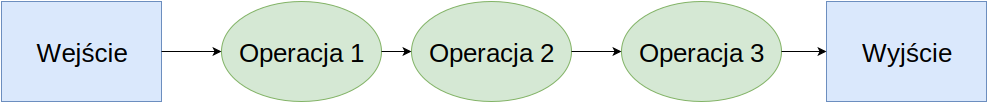
\includegraphics[width=1\textwidth]{img/batch}
	\caption{Procesowanie wsadowe}
  \label{fig:BatchProcessing}
\end{figure}
Takie podejście jest bardzo wygodne z punktu widzenia użytkowania,
po zdefiniowaniu wszystkich operacji oraz dostarczeniu danych wejściowych
proces nie wymaga żadnych dodatkowych czynności ze strony użytkownika.
Dodatkowo z uwagi na swój jednorazowy charakter wiadomo także czy operacje się udały czy nie.

Najpowszechniejszą architekturą wykorzystywaną w przetwarzaniu wsadowym jest \textit{Map Reduce}.
Schemat rozwiązania przedstawiono na rysunku \ref{fig:MapReduce}.
\begin{figure}[htbp]
\centering
	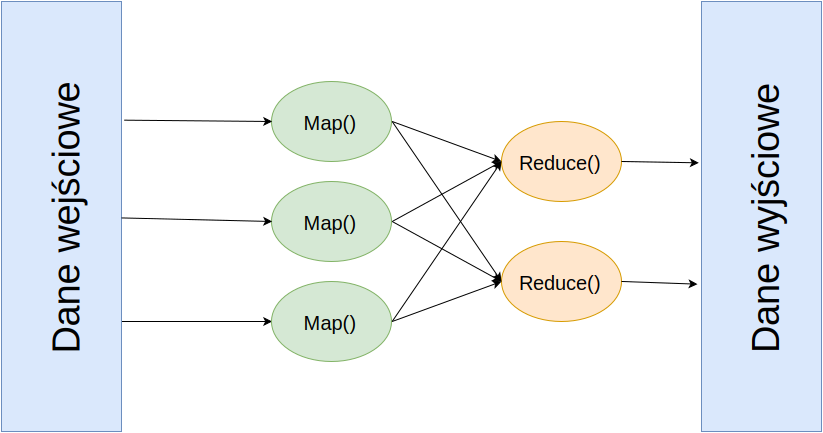
\includegraphics[width=0.9\textwidth]{img/mr}
	\caption{Model architektury rozwiązania \textit{Map Reduce}}
  \label{fig:MapReduce}
\end{figure}
Dane dzielone są na wiele,
niezależnych od siebie zbiorów,
na których wykonywane są różnego rodzaju przekształcenia,
operacje (faza \textbf{Map}).
Po wykonaniu wszystkich obliczeń następuje etap agregowania (faza \textbf{Reduce}) otrzymanych wyników.
Zyski z takiego podejścia najlepiej są widoczne w środowisku rozproszonym (wiele maszyn, procesów i wątków),
gdzie dzięki dekompozycji zadania wzrastają możliwości skalowania.

% TODO:
% Przykłady
% koszyk w supermarkecie

\subsection{Przetwarzanie strumieniowe}

Wymagania użytkowników co do czasu otrzymania wyniku
oraz pewna klasa problemów charakteryzujących się:
\begin{itemize}
	\item dużą szybkością napływania danych -- dane z czujników, sensorów, etc.,
	\item małymi opóźnieniami (\textit{latancy}) podczas procesowani -- wykrywanie oszustw (\textit{fraud detection}),
\end{itemize}
powodują,
że metody przetwarzania wsadowego nie znajdują zastosowania.
Podejście strumieniowe polega na analizie danych bezpośrednio po ich pojawieniu się.
Nie jest istotny sposób w jaki dane się pojawiają,
ale fakt,
że są procesowane natychmiast po pojawieniu się.
Mechanizmy analizy strumieniowej można podzielić na 2 typy z uwagi na sposób przetwarzania:
\begin{itemize}
	\item \textbf{Niezależne}.
	Każdy nowy element (zdarzenie) jest przetwarzany pojedynczo i niezależnie od innych.
	Po wykonaniu operacji przekazywany jest do nowego strumienia bądź umieszczany w strumieniu wyjściowym.
	\item \textbf{Buforowane}.
	Elementy napływające ze strumienia przetrzymywane są przez zdefiniowany okres czasu
	bądź czekają na zebranie wystarczającej liczby elementów.
	Po spełnieniu wymaganego warunku są procesowane
	i tak jak w przypadku procesowania niezależnego	przekazywanie dalej albo na wyjście.
\end{itemize}

% TODO:
% Przykład
